% !TeX root=main.tex
\chapter{مشخصه و دستورالعمل نگارش یک گزارش علمی}\label{Chap:thesis}
\thispagestyle{empty}
این یک توضیح کوتاه است...
\section{مشخصه یک گزارش علمی}
اگرچه برای همه انواع نوشته‌ها، مشخصات و ویژگی‌های واحد و معینی نمی‌توان ذكر كرد، با این حال در یک پایان نامه یا گزارش علمی باید نکات و موارد کلی که در این فصل ذکر می‌شود، بطور کامل رعایت شده باشد. 
دقت كنید كه پس از عنوان فصل باید حداقل توضیحی کوتاه در مورد موضوع نوشته شود و نمی‌توان مستقیماً بعد از آن عنوان بخش را نوشت و همین طور پس از عناوین بخش‌ها و زیربخش‌ها.(مانند دستورالعمل حاضر)
\subsection{برخورداری از غنای علمی }
یك پایان نامه باید پیش از هر چیز به‌لحاظ علمی از غنای لازم برخوردار باشد. یعنی هدف و پیام روشنی داشته باشد و از پیش‌زمینه علمی، بیان دلایل علمی، ارجاعات مورد نیاز و نتیجه‌گیری شفاف بهره ببرد. 
\subsection{ارجاع به‌موقع و صحیح به منابع دیگر}
هر جمله‌ای که در یک پایان نامه نوشته می‌شود یا یک جمله کاملاً بدیهی است یا باید دلیل آن بیان شود و یا اینکه باید به منبعی که آن موضوع را نقل یا اثبات کرده، ارجاع داده شود. اگر مطلب یا گفتاری از منبعی عیناً در گزارش نقل می‌شود، باید آن مطلب داخل گیومه قرار گیرد و با ذكر ماخذ و شماره صفحه، به آن اشاره گردد.
\subsection{ساده‌نویسی}
سادگی از ضروریات یك نوشته است. نویسنده باید ساده، روان و در عین حال شیوا و رسا بنویسد و عبارات مبهم، جملات پیچیده و كلمات نامأنوس در نوشته خود به‌كار نبرد. اگر چه افراط در این امر نیز، به شیوایی نوشته صدمه می‌زند. به‌كارگیری لغات و اصطلاحات دشوار و دور از ذهن و عبارات و جملات نامنظم و مبهم موجب ایجاد اشكال در فهم خواننده خواهد شد‌. 

برای ساده‌نویسی باید در حد امكان از به‌كارگیری كلمات «می‌بایست»، «بایستی»، «گردید»، «بوده باشد» و مانند آنها كه تكلف‌آور، غلط مصطلح و یا غیرشیوا هستند، به‌جای «باید»، «است»، «شد» و مثل آنها، اجتناب شود‌.‌ همین‌طور، «در‌جهت» نمی‌تواند جایگزین خوبی برای كلمه روانی مثل «برای» باشد‌. ‌كلمات و جملات روان و ساده می‌توانند اغلب مفاهیم را براحتی منتقل كنند‌.‌     
 
      دقت در تنظیم بندها (پاراگراف‌ها) نیز كمك شایانی به روانی و سادگی فهم مطلب می‌كند‌.‌ بندهای طولانی نیز مانند جملات طولانی می‌توانند خسته‌كننده باشند و خواننده را سردرگم كنند‌.‌ یك بند نباید کمتر از سه یا چهار سطر یا بیشتر از 10 تا 15 سطر باشد.‌ 
      
\subsubsection{وحدت موضوع}
نویسنده باید در سراسر نوشته از اصل موضوع دور نیافتد و تمام بحث‌ها، مثال‌ها و اجزای نوشته با هماهنگی كامل، پیرامون موضوع اصلی باشد و تاثیری واحد در ذهن خواننده القا كند. 
\subsubsection{ اختصار}
پایان نامه یا گزارش علمی باید در حد امكان، مختصر و مفید باشد و از بحث‌های غیر ضروری در آن پرهیز شود. نوشتن مطالب ارزشمندی كه هیچ ربطی به موضوع ندارد، فاقد ارزش علمی است.
\subsubsection{رعایت نكات دستوری و نشانه‌گذاری}
در سراسر پایان نامه باید قواعد دستوری رعایت شود و اركان و اجزای جمله در جای مناسب خود آورده شود. همچنین رعایت قواعد نشانه‌گذاری سبب می‌شود كه بیان نویسنده روشن باشد و خواننده به سهولت و با کمترین صرف انرژی مطالب را مطالعه و درک كند.
\subsubsection{توجه به معلومات ذهنی مخاطب}
نویسنده باید همواره مخاطب خود را در برابر خود تصور كند و با توجه به معلومات ذهنی مخاطب  تمامی پیش‌نیازهای لازم برای درک مطالب مورد بحث را، از پیش برای مخاطب فراهم كند.
\subsubsection{رعایت مراحل اصولی نگارش}
هر کار علمی زمانی به بهترین شکل قابل انجام است که بر اساس یک برنامه‌ریزی مشخص انجام شود. تهیه یک متن علمی با کیفیت نیز نیازمند برنامه‌ریزی مناسب و اجرای منظم آن می‌باشد. مراحل نگارش را عموماً می‌توان به ترتیب زیر درنظر گرفت:
\begin{itemize}
\item 
	تهیه فهرستی از عناوین اصلی و فرعی که باید نوشته شود
\item 
اولویت‌بندی و تعیین ترتیب منطقی فصل‌ها و بخش‌های گزارش
\item
گردآوری اطلاعات اولیه راجع به هر بخش و زیربخش
\item
تدوین مطالب جدیدی که باید به قلم نگارنده به گزارش اضافه شود
\item
ماشین‌(تایپ)كردن مطالب با رعایت کامل نکاتی که در این دستورالعمل آموزش داده می‌شود
\end{itemize}	
رعایت نظم و ترتیب در اجرای مراحل سیستماتیک فوق هم فرآیند تهیه پایان نامه یا گزارش علمی را برای نگارنده آسان می‌کند و هم کیفیت نگارش را به میزان قابل توجهی افزایش می‌دهد.
\section{نگارش صحیح}
نگارش صحیح یک پایان نامه در فهم آسان آن بسیار موثر است. در این بخش مهمترین قواعد نگارشی که باید مورد توجه جدی نگارنده قرار گیرد، به اختصار بیان می‌شود. این قواعد را می‌توان در محورهای اصلی زیر دسته‌بندی کرد: 
\begin{itemize}
	\item 
	فارسی‌نویسی
	\item
	رعایت املای صحیح
	\item
	رعایت قواعد نشانه‌گذاری
\end{itemize}
\subsection{فارسی‌نویسی}
در حد امكان سعی كنید به جای كلمات غیر‌فارسی از معادل فارسی آنها استفاده كنید، به‌ویژه در مواردی كه معادل فارسی مصطلح و رایج است‌.‌ به‌طور مثال استفاده از كلمه «لذا» به‌جای «برای همین» یا «به‌همین دلیل» توجیهی ندارد‌. همچنین كلمه «پردازش» زیباتر از «پروسس» و معادل فارسی «ریز‌پردازنده» مناسب‌تر از «میكروپروسسور» است‌.‌ در این‌گونه موارد چنانچه احتمال عدم آشنایی خواننده با معادل فارسی وجود دارد، یا اصطلاح غیر‌فارسی معمول‌تر است، در اولین ظهور كلمه فارسی، اصل غیر‌فارسی آن به‌صورت پاورقی آورده شود‌.‌ اگر به‌ناچار باید كلمات انگلیسی در لابه‌لای جملات گنجانده شوند، از هر طرف یك فاصله بین آنها و كلمات فارسی پیش و پس از آنها در‌نظر گرفته شود‌.‌ چنانچه در پایان نامه از مختصر‌نویسی  
\LTRfootnote{Abbreviation}
استفاده شود، لازم است در اولین استفاده، تفصیل آن در پاورقی آورده شود‌.‌ 
مثلاً: همگی می‌دانیم که از سیستم تعیین موقعیت فراگیر 
(\lr{GPS}\LTRfootnote{Global Positioning System})
می‌توان برای تعیین موقعیت جغرافیایی یک وسیله پرنده استفاده کرد.
\subsection{رعایت املای صحیح فارسی}
رعایت املای صحیح فارسی به مطالعه و درك راحت‌تر كمك می‌كند. همچنین در نوشته‌های فارسی باید در حد امكان از همزه « ء، أ، ؤ، ة، إ، ئ» استفاده نشود‌.‌ به‌عنوان مثال «اجزاء هواپیما» و «آئین نگارش» ناصحیح، اما «اجزای هواپیما» و «آیین نگارش» صحیح هستند.‌
\subsection{رعایت قواعد نشانه‌گذاری}
منظور از نشانه‌گذاری به‌كار‌بردن علامت‌ها و نشانه‌هایی است كه خواندن و فهم درست یک جمله را ممکن و آسان می‌كند. در ادامه نشانه‌های معمول و متداول در زبان فارسی و موارد کاربرد آنها به اختصار معرفی می‌شوند.
\subsubsection{ویرگول}
ویرگول نشانه ضرورت یک مكث كوتاه است و در موارد زیر به‌كار می‌رود:
\begin{itemize}
	\item 
	در میان دو كلمه كه احتمال داده شود خواننده آنها را با كسره اضافه بخواند، یا نبودن ویرگول موجب بروز اشتباه در خواندن جمله شود.
	\item
	در موردی كه كلمه یا عبارتی به‌‌‌‌عنوان توضیح، در ضمن یک جمله آورده شود. مثلاً برای کنترل وضعیت فضاپیماها، به‌دلیل آن‌که در خارج از جو هستند، نمی‌توان از بالک‌های آیرودینامیکی استفاده کرد.
	\item
	جدا‌كردن بخش‌های مختلف یك نشانی یا یک مرجع
	\item
موارد دیگر از این قبیل
	پیش از ویرگول نباید فاصله گذاشته شود و پس از آن یك فاصله لازم است و بیشتر از آن صحیح نیست.
\end{itemize}
\subsubsection{نقطه}
نقطه نشانه پایان یک جمله است. پیش از نقطه نباید فاصله گذاشته شود و پس از آن یك فاصله لازم است و بیشتر از آن صحیح نیست. 
\subsubsection{دو نقطه}
موارد كاربرد دونقطه عبارتند از:
\begin{itemize}
	\item 
	پیش از نقل قول مستقیم
	\item 
	پیش از بیان تفصیل مطلبی كه به اجمال به آن اشاره شده ‌است.
	\item 
	پس از واژه‌ای كه معنی آن در برابرش آورده و نوشته می‌شود.
	\item 
	پس از كلمات تفسیر‌كننده از قبیل «یعنی» و ...
\end{itemize}	
پیش از دونقطه نباید فاصله گذاشته شود و پس از آن یك فاصله لازم است و بیشتر از آن صحیح نیست.
\subsubsection{گیومه}
موارد كاربرد گیومه عبارتند از:
\begin{itemize}
	\item 
وقتی كه عین گفته یا نوشته كسی را در ضمن نوشته و مطلب خود می‌آوریم. 
	و در آغاز و پایان كلمات و اصطلاحات علمی و یا هر كلمه و عبارتی كه باید به‌صورت ممتاز از قسمت‌های دیگر نشان داده شود.
	\item
	در ذكر عنوان مقاله‌ها، رساله‌ها، اشعار، روزنامه‌ها و ...
\end{itemize}
\subsubsection{نشانه پرسشی}
پیش از «؟» نباید فاصله گذاشته شود و پس از آن یك فاصله لازم است و بیشتر از آن صحیح نیست. 
\subsubsection{خط تیره}
موارد كاربرد خط تیره عبارتند از:
\begin{itemize}
	\item 
جدا‌كردن عبارت‌های توضیحی، بدل، عطف بیان و ...
	\item 
به‌جای حرف اضافه «تا» و «به» بین تاریخ‌ها، اعداد و كلمات
\end{itemize}
\subsubsection{پرانتز }
موارد كاربرد پرانتز عبارتند از:
\begin{itemize}
\item 
به‌معنی «یا» و «یعنی» و وقتی كه یک كلمه یا عبارت را برای توضیح بیشتر كلام بیاورند.	
\item
وقتی كه نویسنده بخواهد آگاهی‌های بیشتر (اطلاعات تكمیلی) به خواننده عرضه كند.		
\item
		برای ذكر مرجع در پایان مثال‌ها و شواهد.	
\end{itemize}	
\begin{example}
	بین کلمه یا عبارت داخل پرانتز و پرانتز باز و بسته نباید فاصله وجود داشته باشد.
\end{example}

\subsubsection{جدانوشتن كلمات بدون گذاشتن فاصله بین آنها}
گاهی لازم است اجزای یك كلمه از یكدیگر جدا نوشته شوند، بدون آنكه بین آنها فاصله گذاشته شود (مثل كلمه «می‌شود» یا «جدانوشتن»). به این منظور بین دو بخش كلمه مورد نظر از نیم‌فاصله
(\lr{SS})
 استفاده شود. برای ایجاد نیم‌فاصله توسط ویرایشگر 
\lr{TeXstudio}،
ابتدا به منوی 
\begin{latin}
\verb!Macros > Edit Macros...!	
\end{latin}
مراجعه و مانند شکل
\ref{fig:half}
عمل می‌کنیم. در نتیجه با توجه به مرحله چهارم شکل با فشردن کلیدهای
\verb!Ctrl+Shift+2!
می‌توان نیم‌فاصله تولید کرد.
\begin{figure}%[ht]
	\centerline{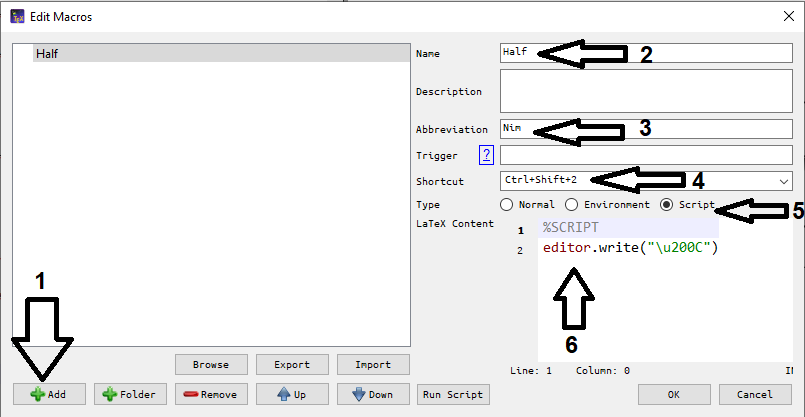
\includegraphics[width=15cm]{images/half}}
	\caption{در این تصویر یک شیر علاقه‌مند به لاتک را در حال دویدن می‌بینید.}
	\label{fig:half}
\end{figure}
 
تقریباً تمامی كلمات مركب در زبان فارسی باید از هم جدا نوشته شوند؛ به استثنای صفات فاعلی مانند «عملگر»، «باغبان» و یا «دانشمند» و كلماتی نظیر «اینكه»، «آنها». در ادامه به نمونه‌هایی از مواردی كه باید اجزای یك كلمه جدا، اما بدون فاصله نوشته شوند، اشاره می‌شود‌.

1-	در افعال مضارع و ماضی استمراری كه با «می» شروع می‌شوند، لازم است كه در عین جدا نوشتن، «می» از بخش بعدی فعل جدا نیافتد‌.‌ برای این منظور باید از «فاصله متصل» استفاده و «می» در اول فعل با SS از آن جدا شود.‌ به‌طور مثال «می‌شود» به‌جای «می شود». 

2-	«ها»ی جمع باید از كلمه جمع بسته‌شده جدا نوشته شود؛ مگر در برخی كلمات مانند «آنها». این امر در مورد كلمات غیر‌فارسی كه وارد زبان فارسی شده‌اند و با حرف «ها» جمع بسته می‌شوند، مانند «كانال‌ها» یا «فرمول‌ها» مورد تاكید است.

3-	حروف اضافه مانند «به» وقتی به‌صورت تركیب ثابت همراه كلمه پس از خود آورده می‌شوند، بهتر است با SS از آن جدا شوند‌.‌ مانند «به‌صورت»، «به‌عنوان» و «به‌‌‌لحاظ»‌.‌ لازم به ذكر است هنگامی كه حرف اضافه «به» با كلمه پس از خود معنای قیدی داشته باشد، مثل «بشدت» یا «بسادگی»، بهتر است كه به‌صورت چسبیده نوشته شود‌.

4-	كلمات فارسی نباید با قواعد عربی جمع بسته شوند؛ پس «پیشنهادها» صحیح و «پیشنهادات» اشتباه است‌.‌

5-	اسم‌ها و صفت‌های دو‌قسمتی مثل «خط‌چین» و «نوشته‌شده» با SS از هم جدا می‌شود‌.‌

6-	شناسه‌ها با SS از كلمه اصلی جدا می‌شود‌.‌ مثل «شده‌اند»‌ و «شده‌است». 

7-	‌ «است» هنگامی كه نقش شناسه را داشته باشد توسط SS از قسمت اصلی جدا می‌شود‌.‌ مانند «گفته‌است»‌.

8-	بند پیشین نباید باعث افراط در استفاده از فاصله متصل شود. مثلاً عبارت «نوشته می‌شود‌« صحیح و عبارت «نوشته‌می‌شود» ناصحیح است. 

9-	فعل‌های دو‌كلمه‌ای كه معنای اجزای آنها كاملاً با معنای كل متفاوت است، بهتر است كه با SS از هم جدا ‌شوند‌.‌

10-	كلمات مركب مثل كلمه «دوكلمه‌ای» در عبارت «فعل‌های دوكلمه‌ای» و «یادداشت‌برداری».

11-	مصدرهای دو قسمتی با SS از هم جدا می‌شوند‌.‌ مثل «ذوب‌كردن» و «واردكردن»‌.

12-	 صفات تفضیلی مثل « آسان‌تر».
